\section{INTRODUCTION}\label{introduction}

% fill missing citations

Most reaching tasks in control and robotics can be phrased as \emph{tracking} problems, where the dynamical system needs to follow a certain predefined trajectory in order to reach a goal state. Robotic table tennis in particular~\cite{Muelling13} consists of planning, generating and executing a series of such (episodic) single stroke trajectories. In order to reach the hitting state precisely, these high-speed trajectories need to be followed with appropriate motor commands. Computing the right motor commands is a nontrivial task when using cable-driven arms such as the Barrett WAM arm shown in Figure~\ref{robot}.

\begin{figure}[t!]
\center
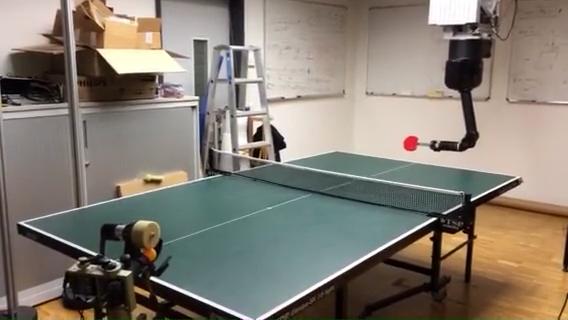
\includegraphics[scale=0.4]{robot1.png}			
\caption{Robotic table tennis setup with the ball-launcher throwing balls to the robot. In order to hit the ball to a desired position on the opponent's court, we give the robot reference trajectories that facilitate the right striking motion. We can teach the robot such trajectories via kinesthetic teach-in.}
\label{robot}
\end{figure}

% maybe cite Jens' review paper
There have been many attempts in the reinforcement learning (RL)~\cite{Sutton98} and control literature to learn robotic tasks directly. Value function based methods take advantage of duality to solve the Bellman's equation but suffer from the initial bias or representation in estimating the value function and do not scale well to high dimensions. Policy search based RL methods (e.g.,~\cite{Kober08}, \cite{Peter10}, \cite{Theodorou10}, \cite{Deisenroth11}) directly solve the Bellman's equation in a parameterized policy space and can be more effective in practice. 
% reference needed for mention of value function approaches

Dynamic Movement Primitives (DMP) are a policy representation that leverages the dynamical systems approach to modify the spring dynamics with a forcing term that enables it to mimic a smooth trajectory. They include an internal phase or clock that ensures the convergence of the movement primitive to a goal state or a limit cycle~\cite{Ijspeert13}. DMPs do not suffer from the curse of dimensionality as the number of parameters (weights) grow linearly with dimension. They can be easily modulated in time and space to allow for variance in motion. However, approximation and control errors in robotic platforms make the application of DMPs less useful in practice. %Small changes to DMPs can often make them more useful.

Motor primitives can be modulated in different ways to adapt to unforeseen events or to ensure the optimal execution of required tasks. They work particularly well with episodic policy search methods that modify the weights of the forcing term based on the rewards received in every episode. By adapting the DMP that was initialized with imitation learning e.g., with kinesthetic teach-in~\cite{Muelling13}, RL approaches are able to achieve complex robotic tasks, such as ball-in-a-cup~\cite{Kober08}. However model-free methods (e.g., \cite{Kober08}, \cite{Peter10}) require many iterations to converge, whereas more data-efficient approaches such as~\cite{Deisenroth11} suffer from computational runtime difficulties and cannot be implemented in real-time robotics tasks. %Optimality of the converged policy cannot be guaranteed by these methods.

% inaccurate ?
Inspired by the successes (and failures) of these previous approaches, the research question that we tackle in this article consists of the following:
%
\begin{itemize}
\item How can we learn to hit optimally, while efficiently exploiting an inaccurate dynamics model in a stable way?
%
\item More specifically, when we have modelling inaccuracies and different initial conditions, how should we learn to track a DMP $\dmp(t)$ such that the robot executes a desired hitting motion, either in table tennis or a similar reaching task e.g., putting in golf?

\end{itemize}
%
%
% maybe include P. Abbeel's work on inaccurate models
\noindent We believe that learning in robotics tasks can be performed much more efficiently by taking advantage of existing imperfect models and demonstrated reference trajectories. 

Iterative Learning Control (ILC) is a fundamental approach in control theory developed to track (time-varying) reference trajectories. It has been used successfully to follow trajectories under unknown repeating disturbances and model mismatch \cite{Bristow06}. In ILC, usually the feedforward control inputs are adjusted after each trial based on the resulting deviations from the reference trajectory. The goal is to drive such deviations to zero. ILC can easily incorporate available dynamics models (e.g. \cite{Moore07}, \cite{Amann95}).
% or equivalently references

In this article, we combine Iterative Learning Control with movement primitives by using ILC as a learning method to track rhythmic DMPs. This way we ensure a safe, reliant and robust way to track reference trajectories and more importantly, to execute hitting and striking motions optimally. We show that the incorporation of DMPs help to make our approach robust to initialization error, i.e. our algorithm generalizes ILC to different initial conditions. As opposed to model-free policy search approaches, we make full use of the nominal rigid body dynamics and inverse dynamics models, which helps us to quickly achieve the desired performance requirements. We validate the performance of the approach in two hitting tasks, and compare with existing methods.
% nominal model instead of known, albeit inexact?

Our contributions can be summarized as follows: we form a link between the ILC literature and the movement primitives by systematically formulating an iterative update for tracking the DMPs. A new and concise formulation of striking primitives with rhythmic DMPs is presented. We form a coherent learning framework and present a new update law for reaching the goal positions and velocities. These are studied in detail and the implemented \emph{goal-based ILC}, or $\alg$ in short, is shown to perform better than the state of the art ILC approaches.

In Section~\ref{relatedWork} we mention related work, especially the state of the art approaches in hitting and reaching tasks. In Section~\ref{problemStatement} we state the problem and introduce our new update law in Section~\ref{method}, relating it to the existing optimization-based ILC approaches. We formulate this update law, called $\alg$, in algorithmic form in Section~\ref{algorithm} and show how it can be used with rhythmic DMPs. In Section~\ref{experiments} we evaluate $\alg$ in robotic table tennis. We show that the method outperforms the state-of-the-art ILC approaches. Finally in Section~\ref{conclusion} we discuss the strengths and weaknesses of our method and conclude with brief mentions of promising future research directions.

\subsection{Related Work}\label{relatedWork}

% mention the ILC paper of Peter Abbeel
Dynamic movement primitives belong to the class of movement primitives~\cite{Flash85}. Movement primitives are a kinematics-based approach to keep the learning tasks in high-dimensional tasks, such as in humanoid robotics, tractable. Like the options framework in Markov Decision Processes~\cite{Sutton99}, they aim at reducing the curse of dimensionality in complex human-like robotics tasks. The first dynamical systems based formulation of movement primitives appeared in~\cite{Ijspeert02}. A good review with alternative and variant formulations is given in~\cite{Ijspeert13}. Discrete DMPs have been extended in \cite{Kober10}, \cite{Muelling13} for striking movements, where the goal state is also evolved in time to allow for high velocities around settling time.

% Policy search methods
%One of the first examples of policy search based methods that modify the parameters of movement primitives is the \emph{POWER} algorithm~\cite{Kober08}. \emph{PI$^{2}$}~\cite{Theodorou10} and episodic-\emph{REPS}~\cite{Peter10} also share similarities with \emph{POWER}.

The work of Arimoto et al.~\cite{Arimoto84} was one of the first to define Iterative Learning Control with the D-type update law. See~\cite{Bristow06} and \cite{Moore07} for reviews. Theoretically, most ILC algorithms can be studied as a \emph{linear repetitive process} using 2D-systems analysis~\cite{Rogers07}. Monotonic convergence and stability guarantees are of central importance for the practical usefulness of ILC algorithms. They are shown for example in~\cite{Bristow06}, \cite{Norrloef02}, \cite{Longman2000}. In practice, some of the assumptions made in the ILC literature may often be violated. Robustness to varying initial conditions are considered e.g., in \cite{Hillenbrand00}, \cite{Park00}, \cite{Fang03}. ILC should be used along with a robust feedback controller to reject nonrepeating disturbances, see e.g., \cite{Chin04},\cite{Longman2000}. 
%Stability analysis of such feedback in the iteration domain has been extended to partially observable environments recently in \cite{Bolder14}. 
%The interested reader can find more references in \cite{Bristow06}, or in \cite{Moore07} where a comprehensive literature review between 1998 and 2004 is given.
% should we cite more authors here about qILC?

% ILC work - mention Angela's work
One of the first papers introducing an optimization based ILC approach incorporating a model of the dynamics is \cite{Amann95}. These methods are closely related to stable plant-inversion approaches~\cite{Ghosh99}. As a more recent example of model-based ILC, Schoellig et al.~\cite{Schoellig12} applied a Kalman-filter based convex optimization rule that avoids direct inversion and showed its performance in quadrocopter flight. An EM-based update law was given in~\cite{Berg10} where an impressive application of ILC to a robotic surgical task was presented. 
% gjm: self-citation here :P
ILC has also been combined with robust observers for controlling a heavy-duty hydraulic arm during excavation tasks~\cite{Maeda2015Combined}. 
% This work however lacks any guarantees of monotonic convergence

% DMPs using Iterative Learning Control
While the large body of ILC literature has almost exclusively addressed invariant reference trajectories, we introduce the use of DMPs as a parameterized trajectory representation, allowing for variations on the desired trajectory and adding more flexibility to controllers based on ILC. DMPs have been also combined in a bimanual robotics task with ILC~\cite{Gams13} where force feedback is used to enable compliant interaction with objects in an unknown environment. ILC is here used to learn a coupling term between the two arm trajectories. In our case we do not change the DMPs but try to track rhythmic DMPs that can succesfully return the ball to the opponent's court.

\subsection{Problem Statement}\label{problemStatement}

The goal in trajectory tracking is to track a given reference $\traj(t), \ 0 \leq t \leq T \ $, in state space $\state \in S \subset \mathbb{R}^{2n}$ by applying the control inputs $\sysInput(t)$. The reference trajectory in our case enables the \emph{optimal} execution of hitting and striking motions, e.g., forehand and backhand strikes in (table) tennis. We assume that such optimal trajectories are available to us, either through kinesthetic teach-in or given a desired Cartesian trajectory, computed recursively using inverse kinematics.
% talk about feasibility.
% reference needed? Dynamic programming?

% subsubsection entitled 'modelling assumptions'?
% talk of model-free regression update of DMP there maybe?
Consider the nonlinear robot dynamics of the form
%
\begin{equation}
\begin{aligned}
\ddot{\joint} &= \dynamics(\joint,\dot{\joint},\sysInput), \\
\ddot{\joint} &= \vec{M}^{-1}(\joint)\{ \vec{\tau}(\sysInput) - \vec{C}(\joint,\dot{\joint})\dot{\joint} - \vec{G}(\joint)\} + \dist(\joint,\dot{\joint}),\\
\end{aligned}
\label{dynamics}
\end{equation}
%
\noindent where on the right hand side are the terms due to the rigid body dynamics model and $\dist(\joint,\dot{\joint})$ are the (unmodeled) disturbances that act on the robot, due to parameter mismatch, viscous friction, stiction, etc. This system can be linearized around a given joint space trajectory $\traj(t), \ 0 \leq t \leq T$ with nominal inputs $\trjInput(t)$ calculated using the inverse dynamics model~\cite{Spong06}. We then obtain the following linear time varying (LTV) representation
%
\begin{equation}
\begin{aligned}
\dot{\error} = \vec{A}(t)\error(t) + \vec{B}(t)\linInput(t) + \linDist(t,\sysInput),
\end{aligned}
\label{LTV}
\end{equation}
%
\noindent where the state error is denoted as $\error(t) = \state(t) - \traj(t)$, the joint angles and velocities are $\state = [\joint^{\intercal},\dot{\joint}^{\intercal}]^{\mathrm{T}}$, $\linInput(t) = \sysInput(t) - \trjInput(t)$ and the continuous time varying matrices are
%
\begin{equation}
\begin{aligned}
\vec{A}(t) &= \at{\frac{\partial{\dynamics}}{\partial{\state}}}{(\traj(t),\trjInput(t))}, \\
\vec{B}(t) &= \at{\frac{\partial{\dynamics}}{\partial{\sysInput}}}{(\traj(t),\trjInput(t))}.
\end{aligned}
\label{LTVmatrices}
\end{equation}
%
% what about estimation errors, i.e. sensor errors ...
\noindent In the error dynamics \eqref{LTV} the additional term $\linDist(t,\sysInput)$ accounts for the disturbances and the effects of the linearization. We can discretize (\ref{LTV}-\ref{LTVmatrices}) with step size $\delta$, $N = T/\delta$ and step index $j = 1, \ldots, N$ to get the following discrete linear system
%
\begin{equation}
\begin{aligned}
\error_{j+1} = \vec{A}_j\error_j + \vec{B}_j\linInput_j + \linDist_j(\sysInput_1, \ldots, \sysInput_j),
\end{aligned}
\label{discreteLTV}
\end{equation}
%
\noindent where the matrices $\vec{A}_j, \vec{B}_j$ are the discretizations of \eqref{LTVmatrices}. Conventional ILC algorithms learn to compensate for the errors by iterating the control inputs $\linInput_j$ with an update law.